\documentclass[]{article}
\usepackage{amsmath}
\usepackage{hyperref}
\usepackage{listings}
\usepackage{graphicx}

%opening
\title{Implementing of a simple Heat-Convection Model}
\author{Florian Nikos Kitzka}

\begin{document}

\maketitle

\begin{abstract}
The aim of this document is to provide a simple guide how to create and implement a model for a heat-convection problem. Our approach is to start from underlying physics to pose the model-equations and then to explain difficulties arising during implementation.
The full implemented result is provided by an external link, which deems to encourage the reader to extend and play with it.
We assume basic knowledge of Analysis and Linear Algebra as well as some understanding of 
Fluid Dynamics. Chapters are written quite independent of each other so that the reader
can skip parts in which no interest exist.
This all deems as an introduction into the subject. Numerical treatment of Fluid Dynamic belongs to one of the most challenging tasks in numerical mathematics.
For the given problem, which is quite easy in each nature our chosen method might work quite satisfactory, but be aware that for other problems much more sophisticated methods are to be taken into consideration.
\end{abstract}

\tableofcontents

\section{Simulation Target}
We consider a room of cubical shape.\\
We assume all walls except the bottom to allow transfer of air (open walls).\\
The bottom is assumed to be heated by the sun-light through radiation.\\
Our goal is to simulate how this heat is being transferred through the room over time.

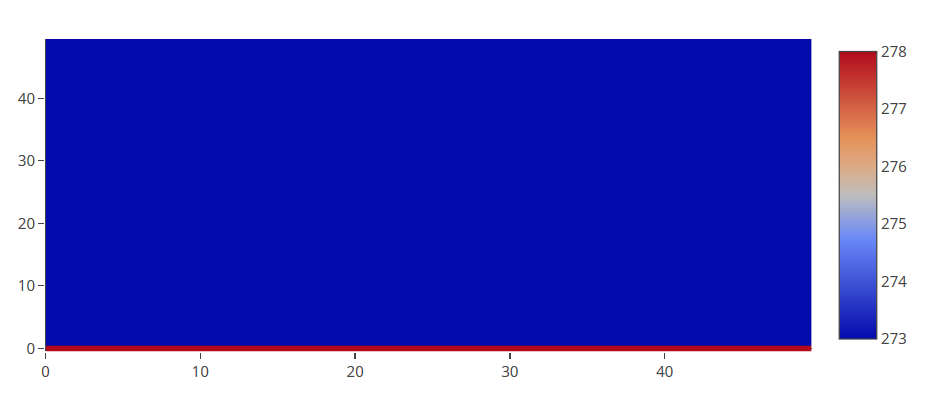
\includegraphics{setup}

\section{Creation of Model} \label{model_creation}
There are two main mechanism of heat transfer in nature. One is diffusion the other is advection. We will shortly explain these two mechanisms and how to incorporate this into a model. For a detailed account on this, the reader is referred to standard literature on Fluid Dynamics.\\
\subsection{Heat Diffusion}
Consider a volume $V$ with edge length $\Delta x$. We denote the temperature at the left surface by $T_L$ and at the right surface by $T_R$. Then Fourier's law states the heat-flux through left surface is
\begin{equation} \label{heat_flux_left}
I(x_0)=-\lambda\frac{\partial T}{\partial x}(x_0)
\end{equation}
and through right surface is
\begin{equation} \label{heat_flux_right}
I(x_1)=-\lambda\frac{\partial T}{\partial x}(x_1)
\end{equation}
$I$ is the amount of heat-energy passing per unit of time through unit of area.
The coefficient $\lambda$ depends on the material.
Furthermore each material which is added heat-energy is changing its temperature according to
\begin{equation*}
c_p \Delta T=\Delta q
\end{equation*}
$q$ denotes the heat-energy per unit of mass and $c_p$ the specific heat capacity. The later depends on the material. By using the density $\rho$ we can rewrite this as
\begin{equation} \label{specific_heat}
c_p \Delta T=\frac{1}{\rho V} \Delta Q
\end{equation}
$Q$ denotes the total heat energy added to the volume $V$.
Analogous consideration as done in (\ref{heat_flux_left}) and (\ref{heat_flux_right}) can be made for all other surfaces. That is, each surface
contributes either positive or negative depending on the direction of flow to the internal change of heat energy per unit of time.
We can formulate this by
\begin{equation*}
\Delta Q = A\Delta t \sum_{j}-I_{j}(x_{j}+\Delta x)+I_{j}(x_{j})
\end{equation*}
where $A$ denotes the area of a surface, $I_{j}(x_j)$ the heat-flux through surface $S_j$
and $I_{j}(x_j+\Delta x)$ the heat-flux through the opposite surface in $V$. Summation is carried out only over the three surfaces which span the volume.
By setting $A=V/\Delta x$ and using equations (\ref{heat_flux_left}), (\ref{heat_flux_right}), (\ref{specific_heat}) in the left and right side correspondingly we obtain
\begin{equation*}
\rho c_p V\Delta T = \lambda A\Delta t\sum_{j}\frac{\partial T}{\partial x_j}(x_j+\Delta x)-\frac{\partial T}{\partial x_j}(x_j)
\end{equation*}
By using $V/A=\Delta x$ this equation is equivalent to
\begin{equation*}
\rho c_p \frac{\Delta T}{\Delta t} = \frac{\lambda}{\Delta x}\sum_{j}\frac{\partial T}{\partial x_j}(x_j+\Delta x)-\frac{\partial T}{\partial x_j}(x_j)
\end{equation*}
At the end we can consider the limit $\Delta x\rightarrow 0$ to find the heat-diffusion equation
\begin{equation}
\frac{\partial T}{\partial t}=\frac{\lambda}{\rho\alpha}\Delta T
\end{equation}
Note, $\Delta T$ refers to the Laplace operator here ($\Delta T=\nabla\cdot\nabla T$).

\subsection{Advection}
Advection describes the mechanism a physical property to be transported by a bulk movement. In our example the bulk movement is presented by the wind and the physical property is either momentum or heat.\\
We consider the same volume $V$ as in previous section and denote the physical (scalar) property by $\phi$. Here $\phi$ shall be given per unit of mass. In addition we denote by $\textbf{v}$ the current velocity field. At the left surface let us consider the normal directed velocity component $v_x$. During the interval $\Delta t$ we have a displacement of mass by
\begin{equation} \label{displacement}
\xi_{x}=v_x\Delta t
\end{equation} 
Thus the net balance of mass flowing into and out of $V$ through the left and right surface is
\begin{equation} \label{net_flow}
-\rho A\cdot\xi_{x+\Delta x} \cdot \phi(x+\Delta x)+\rho A\cdot\xi_{x} \cdot \phi(x)
\end{equation}
which by using (\ref{displacement}) becomes
\begin{equation*}
-\rho A\cdot  v_{x+\Delta x}\cdot\Delta t \cdot \phi(x+\Delta x)+\rho A\cdot  v_{x}\cdot\Delta t \cdot \phi(x)
\end{equation*}
By 'adding a zero' we can rewrite this as
\begin{align*}
&-\rho A\cdot v_{x+\Delta x}\cdot\Delta t \cdot \phi(x+\Delta x) \\ &+
\rho A\cdot v_{x}\cdot\Delta t \cdot \phi(x+\Delta x) -
\rho A\cdot v_{x}\cdot\Delta t \cdot \phi(x+\Delta x) \\ &+
\rho A\cdot v_{x}\cdot\Delta t \cdot \phi(x)
\end{align*}
Further by putting terms together yields
\begin{align*}
&\rho A\cdot (v_{x}-v_{x+\Delta x})\cdot\Delta t \cdot \phi(x+\Delta x) +
\rho A\cdot v_{x}\cdot\Delta t \cdot (\phi(x)-\phi(x+\Delta x))
\end{align*}
By using $A=V/\Delta x$ we can write this as
\begin{align*}
&\rho V \frac{v_{x}-v_{x+\Delta x}}{\Delta x}\cdot\Delta t \cdot \phi(x+\Delta x) +
\rho V v_{x}\cdot\Delta t\frac{\phi(x)-\phi(x+\Delta x)}{\Delta x}
\end{align*}
By letting $\Delta x\rightarrow 0$ we obtain
\begin{equation*}
-\rho \phi(x)\Delta t\cdot V\frac{\partial v_x}{\partial x}
-\rho v_x\Delta t\cdot V \frac{\partial \phi}{\partial x}(x)
\end{equation*}
The same consideration can be done in $y$ and $z$ direction and by adding all these net balances we obtain as net change of $phi$
\begin{equation*}
\rho V \Delta \phi =
-\rho V \Delta t\phi(x)\left(\frac{\partial v_x}{\partial x} 
+\frac{\partial v_y}{\partial y}+\frac{\partial v_z}{\partial z}\right)
 -\rho V \Delta t \left(v_x \frac{\partial \phi}{\partial x}+
 v_y \frac{\partial \phi}{\partial y}+
 +v_z \frac{\partial \phi}{\partial z}\right)
\end{equation*}
Dividing by $\rho V \Delta t$ and letting $\Delta t\rightarrow 0$, we obtain
\begin{equation} \label{transp_equation}
\frac{\partial\phi}{\partial t}=-\phi\nabla\cdot\textbf{v} -\textbf{v}\cdot\nabla\phi
\end{equation}
Note, in very generic contexts one also takes the change of density into account, but here we will assume the density to be global constant.
Also for our needs it will suffice to assume incrompressibility , that is, $\nabla\cdot\textbf{v}=0$. It expresses in essence that all mass flowing into the volume must flow out somewhere else.

We can now use this equation to express transport of heat-energy. Heat-energy and temperature are 
related by $c_p T=u$ where $u$ denotes the inner energy. So what in fact is transported is $u$ and be inserting we get
\begin{equation} \label{transp_heat}
\frac{\partial T}{\partial t}=-\textbf{v}\cdot\nabla T
\end{equation}
Since the moment applies into all three directions we have to consider as $\phi$ separately all components of velocity, $v_x, v_y, v_z$. This gives a set of three equation which we can write compactly as
\begin{equation}
\frac{\partial\textbf{v}}{\partial t}=-\textbf{v}\cdot\nabla\textbf{v}
\end{equation}

\subsection{Momentum Sources}
The initial velocity is assumed to be 0 everywhere. For changes in moment due to Newton it requires a force. For simplification we assume the pressure is in so called hydro-static equilibrium. As only remaining force we consider buoyancy. It always arises when
a region of warmer fluid is surrounded by colder fluid. It only applies in vertical direction and
can be formulated in terms of an acceleration by
\begin{equation}
\textbf{F}_{B}=g\frac{T-T_{A}}{T_{A}}\textbf{e}_{z}
\end{equation}
Here $g$ denotes the gravity acceleration and $T_A$ the surrounding temperature.
For a detailed derivation see standard literature in Fluid Dynamics.
Note, in our implementation we will assume this $T_A$ is just given by the temperature above
the considered grid-point.
\subsection{Final Model}

A final very simplified model looks like this
\begin{align} 
\frac{\partial T}{\partial t}&=-\textbf{v}\cdot \nabla T + \frac{k}{\rho\alpha}\Delta T \label{model_equations} \\
\frac{\partial v_{z}}{\partial t}&=g\frac{T-T_{A}}{T_{A}}-v_{z}\frac{\partial v_{z}}{\partial z} \nonumber
\end{align}

Although we could restrict computation on dimension 1 we will do it for dimension 2 in order to
get more inside into the used techniques.


\section{Numerical Scheme}
In order to solve the model equations (\ref{model_equations}) numerically we are going to use the so called Finite Difference Method. This requires to lay a fixed grid over our domain (the room) and replace all derivative expressions by discrete approximations.\\
Moreover, as we have seen in section \ref{model_creation}, physical properties like
heat and momentum are transported by diffusion and advection processes.\\
Our goal in this section is to provide a generic scheme for both mechanisms.
Hereby we are going to consider both processes independent of each other and restrict
attention to the 1-dimensional case. It will turn out later that this treatment is already
sufficient for the final implementation.\\
A small remark w.r.t our assumed incompressibility condition ($\nabla\cdot\textbf v=0$) must be
maid. Actually after each time-iteration one must ensure these property to be withhold. Usually this is done by adjusting the pressure ('pressure correction'). To simplify things, we will neglect this and assume the pressure and the density to be global constants.

\subsection{Derivative Approximations} \label{derivate_approx}
The main method to obtain such approximations for derivatives is using Taylor expansion.
We give a detailed description for one specific derivative expression but leave the remaining for the reader since they are produced in analogy.\\
Also, for reasons becoming clear later, we restrict our attention to 1-dimensional functions.
Consider the two Taylor expansions,
\begin{equation*}
u(x+h)=u(x)+u'(x)h+\frac{1}{2}u''(x)h^2+o(2)
\end{equation*}
\begin{equation*}
u(x-h)=u(x)-u'(x)h+\frac{1}{2}u''(x)h^2+o(2)
\end{equation*}
By adding both equations we obtain
\begin{equation*}
u(x+h)+u(x-h)=2u(x)+u''(x)h^2
\end{equation*}
By solving the later for $u''(x)$ we get a second-order approximation for the second derivative
of $u$.
\begin{equation*} 
u''(x)=\frac{1}{h^2}(u(x+h)+u(x-h)-2u(x)) + o(2)
\end{equation*}

For the numerical treatment we have to consider $u$ discrete in space and time.
We define 
\begin{equation*}
u_{i}^{n}=u(t_{n}, x_{i})
\end{equation*}
or in case of 2-dimensions
\begin{equation*}
u_{i,j}^{n}=u(t_{n}, x_{i}, y_{j})
\end{equation*}

With this we can now easily list the approximations we are going to use, especially the one
we just obtained for second-order derivatives.

\begin{eqnarray}
	\left[\frac{\partial u}{\partial t}\right]_{i}^{n} & \approx \frac{1}{\Delta t}(u_{i}^{n+1}-u_{i}^{n}) \nonumber  \\
	\left[\frac{\partial u}{\partial x}\right]_{i}^{n} & \approx \frac{1}{\Delta x}(u_{i}^{n}-u_{i-1}^{n})  \label{backward_in_space} \\
	\left[\frac{\partial u}{\partial x}\right]_{i}^{n} & \approx \frac{1}{\Delta x}(u_{i+1}^{n}-u_{i}^{n}) \label{forward_in_space}  \\
	\left[\frac{\partial^2 u}{\partial x^2}\right]_{i}^{n} & \approx
	\frac{1}{\Delta x^2}(u_{i-1}^{n}-2u_{i}^{n}+u_{i+1}^{n}) \nonumber
\end{eqnarray}

For first derivative we have provided two approximations, (\ref{forward_in_space}) is called
forward in space and (\ref{backward_in_space}) is called backward in space.

Note, we only present a small selection of possible ways to approximate derivatives. Also, since this article deems as an introduction we only focused on explicit schemes, but the reader should be aware there exists another important category of so called implicit schemes.
For a more comprehensive list and treatment the reader is referred to standard literature of finite difference method.

\subsection{Advection Scheme}

In general advaction processes have the form
\begin{equation*}
\frac{\partial u}{\partial t} = -c \frac{\partial u}{\partial x} + S
\end{equation*}
Here $S$ denotes a possible source term for the property $u$.\\
By using approximations for derivatives as given in section \ref{derivate_approx}
we can formulate the following scheme:

For positive velocity ($c\geq 0$):
\begin{equation} \label{advection_scheme_upwind}
u_{i}^{n+1}=u_{i}^{n}-c\frac{\Delta t}{\Delta x} (u_{i}^{n}-u_{i-1}^{n}) + S_{i}^{n}
\end{equation}

For negative velocity:
\begin{equation} \label{advection_scheme_downwind}
u_{i}^{n+1}=u_{i}^{n}-c\frac{\Delta t}{\Delta x} (u_{i+1}^{n}-u_{i-1}^{n}) +S_{i}^{n}
\end{equation}

The reason for splitting the scheme based on the direction of velocity becomes clear in section \ref{stability}.

\subsection{Diffusion Scheme}
Diffusion processes are of the form
\begin{equation*}
\frac{\partial u}{\partial t} = \alpha \frac{\partial^2 u}{\partial x^2}
\end{equation*}
and again by using derivative approximations from section \ref{derivate_approx} we
formulate the following scheme:
\begin{equation} \label{diffusion_scheme}
u_{i}^{n+1}=u_{i}^ {n}+\alpha\frac{\Delta t}{\Delta x^{2}} (u_{i-1}^{n}-2u_{i}^{n}+u_{i+1}^{n})
\end{equation}

\subsection{Stability} \label{stability}
One of the most important things with the use of approximation
schemes is to ensure stability.
Actually one could argue that since we have justified all our derivative approximations by Taylor-expansions we are ready and can blindly implement the discrete equations into 
a computer-system. This approach turns out to be too naive.\\
In general each computation is accompanied with rounding errors. Although these can be very small they can sum-up drastically when we have to repeat calculations iterative.
Our scheme has the form 
\begin{equation} \label{stability_scheme}
u_{n+1}=A(u_{n})
\end{equation}
where $A$ is some linear function. \\
If we assume the $u_{n}$'s to be computed without rounding errors (hypothetically), and our 
'realistic' calculated values are $\tilde{u}_{n}$ then we have
\begin{equation}
\tilde{u}_{n}=u_{n}+\epsilon_{n}
\end{equation}
where $\epsilon_{n}$ denotes the deviation of step $n$.
Therefore instead of (\ref{stability_scheme}) we actually deal with
\begin{equation} \label{deviated_scheme}
u_{n+1}+\epsilon_{n+1}=A(u_{n}+\epsilon_{n})
\end{equation}
We observe, at step $n$ we obtained a deviated solution which we use to compute step $n+1$.
Thus at step $n+1$ we are faced to the rounding error made in this step and the fact that we
were actually using the deviated solution, $u_{n}+\epsilon_{n}$, as input.
So the very important question arises: How does the $\epsilon_{n}$'s evolve over time?\\
Combining equations (\ref{stability_scheme}), (\ref{deviated_scheme}) and using linearity of $A$ we obtain
\begin{equation} \label{error_scheme}
\epsilon_{n+1}=A(\epsilon_{n})
\end{equation}
This gives us a direct relation between errors at different steps.
The striking idea is to formulate a scheme, that is choose $A$, so that for all $n$
\begin{equation} \label{scheme_error}
|\epsilon_{n+1}| \leq |\epsilon_{n} |
\end{equation}
Note, if above equation holds, then we can be sure that although we still have to face 
rounding errors, the fact that we use a deviated version, $u_{n}+\epsilon_{n}$, as input in
step $n+1$ does not impact the overall outcome of the iteration.\\
In order to show a given scheme to fulfill (\ref{scheme_error}) we use a method invented by John von Neumann.\\
The idea behind this is to assume the errors can be approximated (or estimated) by a Fourier-expansion
\begin{equation} \label{error_fourier_exp}
\epsilon(t,x)=e^{at}\sum_{k}e^{jkx}
\end{equation}
In other words, some function which decreases or increases exponentially in time. Our aim is to find a scheme $A$ which enforces $a<0$ in above representation of $\epsilon(t,x)$.\\

\subsubsection{Diffusion Scheme}
We replace $\epsilon(t,x)$ in equation (\ref{scheme_error}) by using for $A$ the scheme given in (\ref{diffusion_scheme}). Since $A$ is linear we can restrict attention to one specific index $k$ in (\ref{error_fourier_exp}) to obtain
\begin{equation*}
e^{a(t+\Delta t)}e^{jkx_{i}}=e^{at}e^{jkx_{i}}+\alpha\frac{\Delta t}{\Delta x^2}
\left(e^{at}e^{jk(x_{i}-\Delta x)} -2e^{at}e^{jkx_{i}}+e^{at}e^{jk(x_{i}+\Delta x)}\right)
\end{equation*}
Note the we have used $x_{i-1}=x_{i}-\Delta x$, $x_{i+1}=x_{i}+\Delta x$ and $\epsilon(t_{n+1}, x_{i})=\epsilon(t_{n}+\Delta t, x_{i})$.\\
Further by canceling out factors on both sides we get
\begin{equation*}
e^{a\Delta t}=1+\alpha\frac{\Delta t}{\Delta x^2}
\left(e^{-jk\Delta x} -2+e^{jk\Delta x}\right)
\end{equation*}
Further by use of Euler's formula the r.h.s can be combined to get
\begin{equation*}
e^{a\Delta t}=1+\alpha\frac{\Delta t}{\Delta x^2}
\left(2cos(k\Delta x) -2\right)
\end{equation*}
Since the $cos$ always has absolute values below $1$ we infer a sufficient condition the l.h.s to be lower $1$ is $2\alpha\frac{\Delta t}{\Delta x^2}\leq\frac{1}{2}$ or equivalently,
\begin{equation} \label{stability_restr_diffusion}
\Delta t\leq \frac{1}{4}\frac{\Delta x^2}{\alpha}
\end{equation}
In other words, in order to ensure our diffusion-scheme to be stable, we have to impose (\ref{stability_restr_diffusion}) onto our implementation - we cannot choose arbitrary large time steps $\Delta t$ for given a grid-width $\Delta x$.

\subsubsection{Advection Scheme}
The same steps as above but by using as $A$ the scheme (\ref{advection_scheme_upwind}) we obtain
\begin{equation*}
e^{at}=1-c\frac{\Delta t}{\Delta x}\left(1-e^{-jk\Delta x}\right)
\end{equation*}
We can use the triangle inequality to estimate
\begin{equation*}
e^{at}\leq \left|1-c\frac{\Delta t}{\Delta x}\right| + c\frac{\Delta t}{\Delta x}
\end{equation*}
Note, we have used the known identity $|e^{jy}|=1$.\\
From the we can conclude the r.h.s to be lower $1$ if $0\leq c\Delta t/\Delta x\leq 1$ or equivalent
\begin{equation} \label{stability_crit_advect}
\Delta t\leq \frac{\Delta x}{c}
\end{equation}
For the case of $c<0$ above consideration would show scheme (\ref{advection_scheme_upwind}) to never be stable. But if the same steps as above are applied on scheme (\ref{advection_scheme_downwind}) instead we find the same stability criterion (\ref{stability_crit_advect}).

\subsection{Operator and Term Splitting}
You might have wondered that our approximation schemes all were targeted at 1-dimensional problems, but our model is formulated in two dimensions. Moreover
we have treated diffusion and advection independent of each other whereas in our
model they interact with each other.\\
The secrete behind this is an elegant trick referred as Operator and Term Splitting which allows us in the final implementation to separate dimensions and
transport mechanisms. In other words we can implement for each dimension and each
transport mechanism a scheme and then combine these schemes with each other.\\

\subsubsection{Dimensional Split}
Let us use the advection-scheme as explanatory example. Once understanding the idea, the reader easily can adapt the techniques to other schemes.\\
We can write scheme (\ref{advection_scheme_upwind}) in an operator form
\begin{equation*}
L_{x} := id - c\Delta t \delta_{x}+S
\end{equation*}
Hereby $\delta_{x}$ stands for an operator which takes a function $u$ as argument and 
returns the approximated first derivative on a given grid, that is
\begin{equation*}
\delta_{x}(u_{i}) = \frac{u_{i}-u_{i-1}}{\Delta x}
\end{equation*}
Further $id$ denotes the identity operator
\begin{equation*}
id(u_{i})=u_{i}
\end{equation*}
 and $S$ a constant operator
\begin{equation*}
S(u_{i})=S_{i}
\end{equation*}
With this definitions our scheme (\ref{advection_scheme_upwind}) can be written as
\begin{equation*}
u^{n+1}_{i} = L_{x}(u^{n}_{i})
\end{equation*}
In analogy we can define the operator $L_{y}$ which applies in $y$-direction
\begin{equation*}
L_{y}:=id - c\Delta t \delta_{y}+S
\end{equation*}
and compute the composition of both
\begin{equation} \label{L_x_comp_L_y}
L_{x}\circ L_{y}=id-c\Delta t\delta_{x}-c\Delta t\delta_{y}+o(2)
\end{equation}
In the later we have skipped terms of order $2$ in $\Delta t$.
The general advaction-process in dimension 2 has the form,
\begin{equation*}
\frac{\partial u}{\partial t} = -c_{x}\frac{\partial u}{\partial x}-c_{y} \frac{\partial u}{\partial y}
\end{equation*}
We can use derivative approximations from section \ref{derivate_approx} to obtain a scheme in the form
\begin{equation} \label{L_xy_scheme}
u_{i,j}^{n+1}=u_{i,j}^{n}-c_{x}\frac{\Delta t}{\Delta x}(u_{i,j}^{n}-u_{i-1,j}^{n})
-c_{y}\frac{\Delta t}{\Delta x}(u_{i,j}^{n}-u_{i,j-1}^{n})
\end{equation}
Now it is an easy task to verify that 
\begin{equation*}
L_{x}\circ L_{y}(u_{i,j})=u_{i,j}^{n}-c_{x}\frac{\Delta t}{\Delta x}(u_{i,j}^{n}-u_{i-1,j}^{n})
-c_{y}\frac{\Delta t}{\Delta x}(u_{i,j}^{n}-u_{i,j-1}^{n}) +o(2)
\end{equation*}
and by comparing with (\ref{L_xy_scheme}) to see that the 2-dimensional scheme coincides 
up to order 2 with the composition of the 1-dimensional scheme.\\
Therefore, in our implementation instead of writing the scheme (\ref{L_xy_scheme}) we will first apply the advection scheme (\ref{advection_scheme_upwind}) for $x$-direction and on the result we will again apply (\ref{advection_scheme_upwind}) but in $y$-direction.

\subsubsection{Term Splitting}
The idea of term splitting is quite the same as for dimension splitting. But this times the split is done w.r.t different physical processes, that is diffusion and advection.\\
Like for the advection scheme we can introduce an operator which describes scheme (\ref{diffusion_scheme})
\begin{equation*}
L_{d}:=id+\alpha\Delta t\delta_{xx}
\end{equation*}
whereas
\begin{equation*}
\delta_{xx}(u_{i})=\frac{u_{i-1}-2u_{i}+u_{i+1}}{\Delta x^2}
\end{equation*}
When we compose $L_{d}$ with $L_{x}$ from previous section we obtain
\begin{equation*}
L_{x}\circ L_{d}=id-c\Delta t\delta_{x}+\alpha\Delta t\delta_{xx}+o(2)
\end{equation*}
A system containing diffusion and advection has in general the form
\begin{equation*}
\frac{\partial u}{\partial t} = -c\frac{\partial u}{\partial x}+\alpha\frac{\partial^2 u}{\partial x^2}
\end{equation*}
Again we can use the derivative approximations from section \ref{derivate_approx} to obtain a scheme
\begin{equation} \label{diff_adv_scheme}
u_{i}^{n+1}=u_{i}^{n}-c\Delta t\delta_{x}(u_{i}^{n})+\alpha\Delta t\delta_{xx}(u_{i}^{n})
\end{equation}
We observe that the composition $L_{x}\circ L_{d}$ coincides up to order 2 with above scheme.\\
So, in implementation instead of writing (\ref{diff_adv_scheme}) we will first apply $L_{d}$ and on the result $L_{x}$.

\subsection{Final Scheme}
In previous sections we were describing things a little bit more general than they actually are in our specific model. Since buoyancy only acts into $y$-direction we have only the $z$-component of velocity to have a positive value. Due to our specific boundary conditions we actually could model the entire system in 1-dimension but for educational reasons we do it in 2-dimensions.\\
How final scheme can be written by using above operator expressions as
\begin{equation} \label{final_scheme_expr}
u_{i,j}^{n+1}=L_{x}\circ L_{D,y}\circ L_{D,x}(u_{i,j}^{n})
\end{equation}
$L_{D,x}$, $L_{D,y}$ denote the 1-dimensional diffusion operators applied in $x$-direction resp. $y$-direction.\\
This is an explicit scheme which becomes very handy to implement in this form as we will see next.

\section{Implementation}
This section will explain the important snippets of code which can be found at \url{https://github.com/applied-math-coding/basic-diffusion-transport}. \\
Implementation is provided in Typescript (by utilizing the package [TODO lina]) and in Python.
An online running example can be found here,\\
 \url{https://applied-math-coding.github.io/basic-diffusion-transport/}.
We will give detailed explanations for the Python code only. The Typescript code is similar structured and due to the use of [TODO lina] operator implementation are quite straight forward.\\

Model parameter are defined in the file 'params.py'.
We initialize the temperature and velocity field by using three matrices. Note, the matrices
include the boundaries:
\begin{lstlisting}[language=Python]
T = np.empty((params.n_grid, params.n_grid))
T.fill(params.T_c)
v_y = np.zeros((params.n_grid, params.n_grid))
v_x = np.zeros((params.n_grid, params.n_grid))
\end{lstlisting}

We iterate the application of all operators and ensure the results are directly written
into above matrices:
\begin{lstlisting}[language=Python]
def simulate():
  t = 0
  while t <= params.duration:
    utils.adjust_boundary(T, v_x, v_y)
    utils.diffusion_x_op(T, alpha, delta_t, delta_x)
    utils.diffusion_y_op(T, alpha, delta_t, delta_x)
    utils.heat_convection_y_op(T, v_y, delta_t, delta_x)
    utils.mom_convection_y_op(T, v_y, delta_t, delta_x)
    utils.adjust_boundary(T, v_x, v_y)
    t = t+delta_t
\end{lstlisting}

Each operator is defined in file 'utils.py'.
The boundary conditions are ensured by:
\begin{lstlisting}[language=Python]
def adjust_boundary(T, v_x, v_y):
  T[0, :] = params.T_h
  T[-1, :] = T[-2, :]
  T[:, 0] = T[:, 1]
  T[:, -1] = T[:, -2]
  v_y[0, :] = 0
  v_y[-1, :] = v_y[-2, :]
  v_y[:, 0] = v_y[:, 1]
  v_y[:, -1] = v_y[:, -2]
\end{lstlisting}

In order to implement the operators, instead of using loops we are element-wise combining (adding, ...) matrices which indexes are shifted correspondingly in order to achieve the 
specific schemes receipt (note how much the implementation resembles the actual scheme's definition):
\begin{lstlisting}[language=Python]
def diffusion_x_op(T, alpha, delta_t, delta_x):
  T[1:-1, 1:-1] = T[1:-1, 1:-1] + alpha * delta_t / \
  pow(delta_x, 2)
    * (T[1:-1, 0:-2]-2*T[1:-1, 1:-1]+T[1:-1, 2:])


def diffusion_y_op(T, alpha, delta_t, delta_x):
  T_cen = T[1:-1, 1:-1]
  T_down = T[0:-2, 1:-1]
  T_up = T[2:, 1:-1]
  T[1:-1, 1:-1] = T_cen + alpha * delta_t / \
  pow(delta_x, 2) * (T_down-2*T_cen+T_up)


def heat_convection_y_op(T, v_y, delta_t, delta_x):
  T_cen = T[1:-1, 1:-1]
  T_down = T[0:-2, 1:-1]
  v_y_cen = v_y[1:-1, 1:-1]
  T[1:-1, 1:-1] = T_cen - delta_t / delta_x * v_y_cen
    * (T_cen-T_down)


def mom_convection_y_op(T, v_y, delta_t, delta_x):
  T_cen = T[1:-1, 1:-1]
  v_y_cen = v_y[1:-1, 1:-1]
  v_y_down = v_y[0:-2, 1:-1]
  T_up = T[2:, 1:-1]
  b = params.g * np.maximum(np.zeros(T_cen.shape),
  (T_cen-T_up)/T_up)
  v_y[1:-1, 1:-1] = v_y_cen + delta_t * b - \
  delta_t / delta_x * v_y_cen * (v_y_cen-v_y_down)
\end{lstlisting}

\section{Further Reading}
This article intends to give an introduction into all treated areas.
There are many good books or only tutorials about numerical treatment of partial
differential equations. Or if you are more specialized on fluid dynamics you will
many good accounts on this field too. In case your are more interested in the 
implementation side, be encouraged to clone the entire project from
\url{https://github.com/applied-math-coding/basic-diffusion-transport} and to extend or play around.
\end{document}
